\chapter{Discussion}\label{chapter:discussion}

One aim of the master thesis was to investigate whether GraphQL with a shared caching layer and query reduction can improve performance in micro-frontend architectures. The improvement should be accomplished using a single caching layer for all micro-frontends and a mechanism to reduce queries by utilizing the in-memory cache structure. The technology-agnostic and prototypical implementation of the micro-frontends is further discussed in this chapter. The results of evaluating the caching improvements of the prototypical micro-frontend implementation architecture are also discussed in this chapter. The findings of Chapter \ref{chapter:results} are used to make a statement about the hypothesis from Chapter \ref{chapter:introduction}. The next following sections focus on discussing the results in terms of request size and response size. The chapter closes by comparing the total time to fetch all responses from the \ac{BFF}.

\section{Request Size}\label{section:discussion:request-size}

This section compares the different measurements of the request sizes from Chapter \ref{chapter:results}. Figure \ref{fig:discussion:request-size} displays the results from the previous sections \ref{section:results:comparison-first-journey} and \ref{section:results:comparison-second-journey} as a bar chart for better comparison. As shown in the figure for the first user journey the differences in request sizes are not very significant. The third approach with no query reduction and no shared cache is the largest, but it executes 11 more requests than the other two approaches. These 11 extra GraphQL queries make up the total difference from the second approach with just the shared caching layer because the queries are not reduced by using the cache. The difference between the first and the second approach is only 1.65 KB. 

\bigskip

\noindent The second user journey shows a quite similar result. In the second approach compared to the third, 25 requests are omitted, by just using a shared caching layer. These differences in requests result in a greater difference in request sizes, which is about 6.07 KB. But again the difference from the first approach to the second approach is not very large, as it is again about 2.17 KB. The difference between the first and second approaches comes only from the omitted fields in the query. The difference of 2.17 KB is quite small compared to the 37 GraphQL queries that executed against the \ac{BFF}.

\bigskip

\noindent Therefore, the query reduction does not make a significant improvement by reducing the size of the requests in comparison to just using the shared caching layer.

\begin{figure}[H]
  \centering
  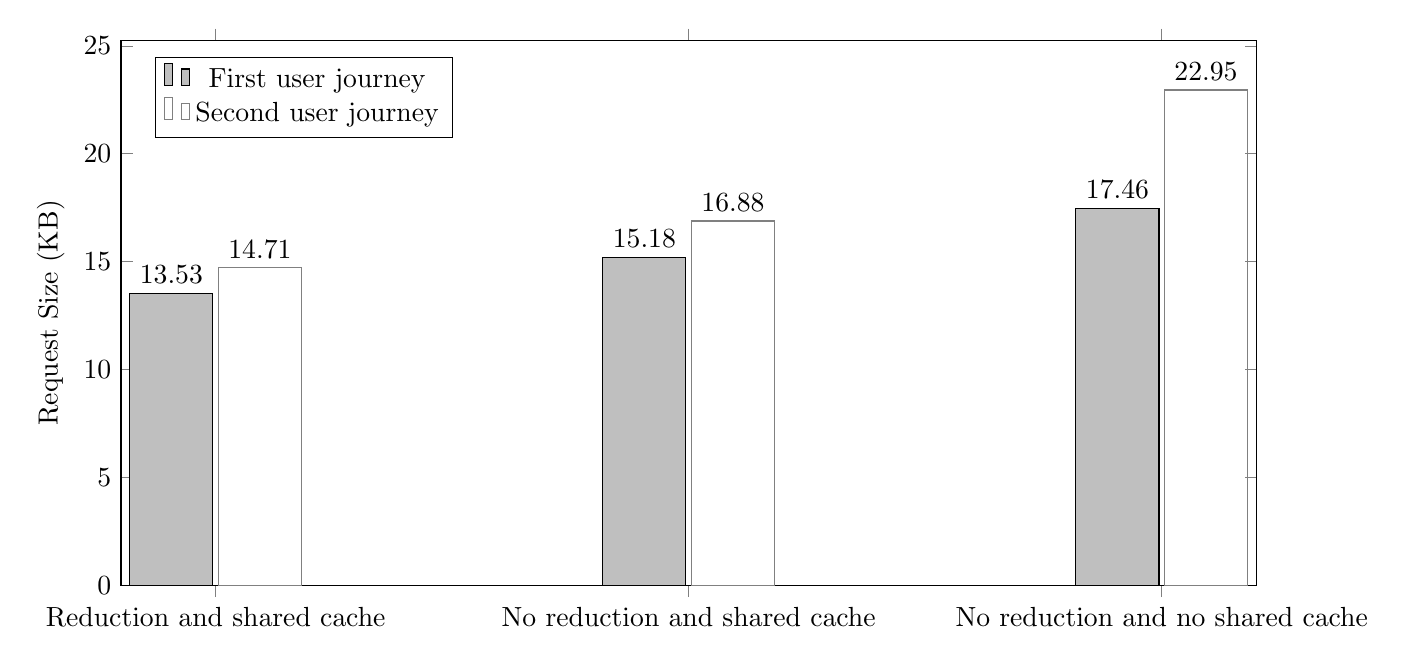
\begin{tikzpicture}
    \begin{axis}[
      ymin=0,
      ybar,
      legend pos=north west,
      ylabel={Request Size (KB)},
      xtick=data, 
      symbolic x coords={Reduction and shared cache, No reduction and shared cache, No reduction and no shared cache}, 
      nodes near coords align={vertical},
      nodes near coords,
      height=8.5cm,
      width=16cm,
      bar width=30pt,
      cycle list={
        {fill=lightgray, draw=gray}
      },
    ]
    \addplot coordinates {(Reduction and shared cache, 13.53) (No reduction and shared cache, 15.18) (No reduction and no shared cache, 17.46)};
    \addplot coordinates {(Reduction and shared cache, 14.71) (No reduction and shared cache, 16.88) (No reduction and no shared cache, 22.95)};
    \legend{First user journey, Second user journey}
    \end{axis}
  \end{tikzpicture}
  \caption{Request size comparison between the three approaches.}\label{fig:discussion:request-size}
\end{figure}

\noindent The next section compares the response sizes of the GraphQL \ac{API} of the three approaches.

\section{Response Size}\label{section:discussion:response-size}

This section compares the response sizes from the GraphQL \ac{API} of the three approaches. Figure \ref{fig:discussion:response-size} displays the results already shown in the previous sections \ref{section:results:comparison-first-journey} and \ref{section:results:comparison-second-journey} as a bar chart for better comparability. Clearly, visible is that the differences in response size are more significant than the difference in request size. As displayed in the figure, the difference between the approach with no query reduction and no shared cache is about 2.35 MB. Therefore, the 11 requests that are committed by using the shared caching are responsible for more than 2 MB of data that needs to be downloaded unnecessarily. This difference could make a huge difference in page performance when using a mobile device. The difference between the first and second approaches is only about 62 KB, which is not very significant and does not make a real difference. Saving 62 KB of data in 37 GraphQL queries is not worth the effort of implementing and using the query reduction. 

\bigskip

\noindent The second user journey shows a quite similar outcome, as the size differences are quite similar. The second approach in the second user journey omits 25 requests in comparison to the naive third approach. This results again in a difference of about 2.35 MB. There is just a 3 KB difference in response sizes between the first and second approaches. These differences are coming from the omitted fields from queries, which is quite small compared to the 37 GraphQL queries that are executed against the \ac{BFF}.

\bigskip

\noindent Just like with the request sizes, the query reduction does not make a significant improvement by reducing the size of the responses in comparison to just using the shared caching layer.

\begin{figure}[H]
  \centering
  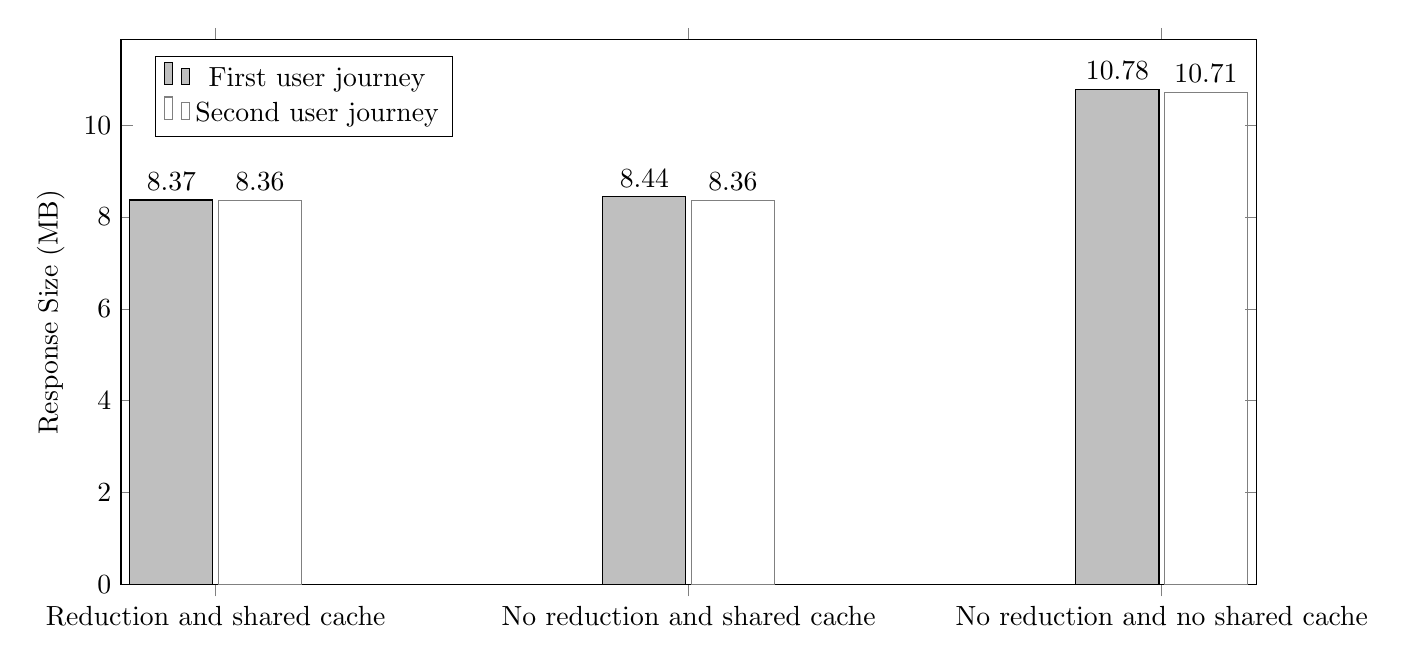
\begin{tikzpicture}
    \begin{axis}[
      ymin=0,
      ybar,
      legend pos=north west,
      ylabel={Response Size (MB)},
      xtick=data, 
      symbolic x coords={Reduction and shared cache, No reduction and shared cache, No reduction and no shared cache}, 
      nodes near coords align={vertical},
      nodes near coords,
      height=8.5cm,
      width=16cm,
      bar width=30pt,
      cycle list={
        {fill=lightgray, draw=gray}
      },
    ]
    \addplot coordinates {(Reduction and shared cache, 8.37) (No reduction and shared cache, 8.44) (No reduction and no shared cache, 10.78)};
    \addplot coordinates {(Reduction and shared cache, 8.361) (No reduction and shared cache, 8.364) (No reduction and no shared cache, 10.71)};
    \legend{First user journey, Second user journey}
    \end{axis}
  \end{tikzpicture}
  \caption{Response size comparison between the three approaches.}\label{fig:discussion:response-size}
\end{figure}

\noindent The next section takes the response into perspectives and compares the response times of the three approaches. This is important because smaller responses lead to faster responses, which is a crucial factor for the user experience.

\section{Response Times}\label{section:discussion:response-times}

It is hard to make real comparisons when it comes to measuring the time it takes to fetch the responses from the backend. The network speed can vary greatly over time, therefore it is not easy to make a reproducible comparison. Therefore, the measurement was done using the throttle mode inside the \href{https://developer.chrome.com/docs/devtools/}{Google DevTools}. The network speed was set to 1.5 Mbps also named \enquote{fast 3G} preset inside the developer tools. This ensures that the network speed stayed the same for all three approaches. The response times were measured three times for every approach and the mean value was taken to get a neutral value. The preset \enquote{fast 3G} was chosen because it is quite slow and makes it possible for times to differ more significantly. With faster network speeds, the differences would be smaller and harder to compare in general. And 3G is still a quite common network speed for mobile connections in many countries. 

\bigskip

\noindent This section measures the total time to download every query response from the GraphQL \ac{API} for the three approaches from section \ref{section:results:performance-measurement}. The measurement must not be misunderstood, because the browser loads the resources partially in parallel. Here only total download time is measured to see how much time is needed to download all the resources in one of the approaches. The measurements were recorded during the user journeys from section \ref{section:results:comparison-first-journey} and \ref{section:results:comparison-second-journey} alongside the request sizes and response sizes. Therefore the total response times correspond to the measured network sizes from the previous two chapters. The results are measured in seconds and are shown in figure \ref{fig:discussion:response-times}. The speeds

\begin{figure}[H]
  \centering
  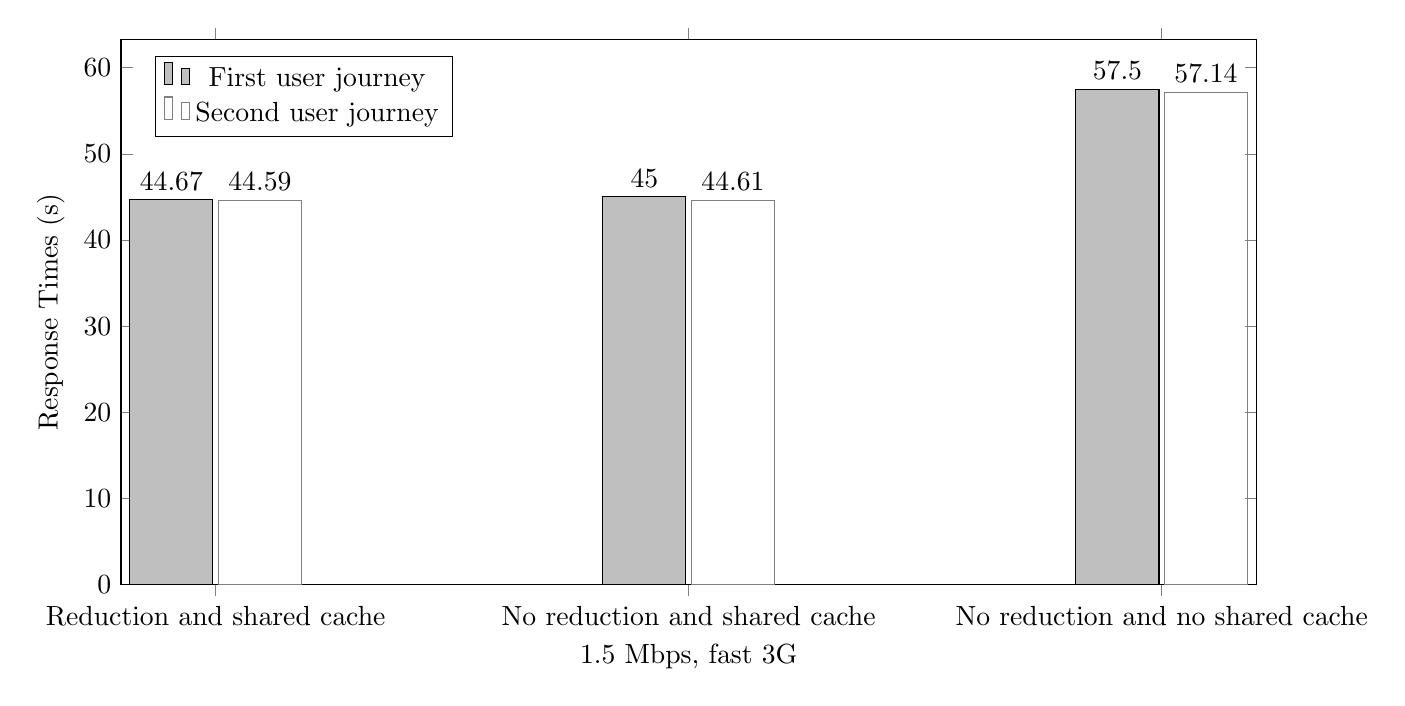
\begin{tikzpicture}
    \begin{axis}[
      ymin=0,
      ybar,
      legend pos=north west,
      ylabel={Response Times (s)},
      xlabel={1.5 Mbps, fast 3G},
      xtick=data, 
      symbolic x coords={Reduction and shared cache, No reduction and shared cache, No reduction and no shared cache}, 
      nodes near coords align={vertical},
      nodes near coords,
      height=8.5cm,
      width=16cm,
      bar width=30pt,
      cycle list={
        {fill=lightgray, draw=gray}
      },
    ]
    \addplot coordinates {(Reduction and shared cache, 44.67) (No reduction and shared cache, 45.00) (No reduction and no shared cache, 57.50)};
    \addplot coordinates {(Reduction and shared cache, 44.59) (No reduction and shared cache, 44.61) (No reduction and no shared cache, 57.14)};
    \legend{First user journey, Second user journey}
  \end{axis}
  \end{tikzpicture}
  \caption{Response time comparison between the three approaches.}\label{fig:discussion:response-times}
\end{figure}

\noindent Like before, the difference between the second approach and the third approach is quite significant. The second approach for both journeys is about 12 seconds faster than the third approach. The eleven respectively 25 requests that are omitted by using the shared caching layer are responsible for about 12 seconds of extra download time. The results from this measurement correspond to the response size measurement from the previous section \ref{section:discussion:response-size}. The results for both the first approach and the second approach are practically the same. The reduction of 37 queries does not yield the expected results and does not speak in favor of using query reduction.